% Options for packages loaded elsewhere
\PassOptionsToPackage{unicode}{hyperref}
\PassOptionsToPackage{hyphens}{url}
%
\documentclass[
  landscape]{article}
\usepackage{amsmath,amssymb}
\usepackage{iftex}
\ifPDFTeX
  \usepackage[T1]{fontenc}
  \usepackage[utf8]{inputenc}
  \usepackage{textcomp} % provide euro and other symbols
\else % if luatex or xetex
  \usepackage{unicode-math} % this also loads fontspec
  \defaultfontfeatures{Scale=MatchLowercase}
  \defaultfontfeatures[\rmfamily]{Ligatures=TeX,Scale=1}
\fi
\usepackage{lmodern}
\ifPDFTeX\else
  % xetex/luatex font selection
\fi
% Use upquote if available, for straight quotes in verbatim environments
\IfFileExists{upquote.sty}{\usepackage{upquote}}{}
\IfFileExists{microtype.sty}{% use microtype if available
  \usepackage[]{microtype}
  \UseMicrotypeSet[protrusion]{basicmath} % disable protrusion for tt fonts
}{}
\makeatletter
\@ifundefined{KOMAClassName}{% if non-KOMA class
  \IfFileExists{parskip.sty}{%
    \usepackage{parskip}
  }{% else
    \setlength{\parindent}{0pt}
    \setlength{\parskip}{6pt plus 2pt minus 1pt}}
}{% if KOMA class
  \KOMAoptions{parskip=half}}
\makeatother
\usepackage{xcolor}
\usepackage[margin=1in]{geometry}
\usepackage{color}
\usepackage{fancyvrb}
\newcommand{\VerbBar}{|}
\newcommand{\VERB}{\Verb[commandchars=\\\{\}]}
\DefineVerbatimEnvironment{Highlighting}{Verbatim}{commandchars=\\\{\}}
% Add ',fontsize=\small' for more characters per line
\usepackage{framed}
\definecolor{shadecolor}{RGB}{248,248,248}
\newenvironment{Shaded}{\begin{snugshade}}{\end{snugshade}}
\newcommand{\AlertTok}[1]{\textcolor[rgb]{0.94,0.16,0.16}{#1}}
\newcommand{\AnnotationTok}[1]{\textcolor[rgb]{0.56,0.35,0.01}{\textbf{\textit{#1}}}}
\newcommand{\AttributeTok}[1]{\textcolor[rgb]{0.13,0.29,0.53}{#1}}
\newcommand{\BaseNTok}[1]{\textcolor[rgb]{0.00,0.00,0.81}{#1}}
\newcommand{\BuiltInTok}[1]{#1}
\newcommand{\CharTok}[1]{\textcolor[rgb]{0.31,0.60,0.02}{#1}}
\newcommand{\CommentTok}[1]{\textcolor[rgb]{0.56,0.35,0.01}{\textit{#1}}}
\newcommand{\CommentVarTok}[1]{\textcolor[rgb]{0.56,0.35,0.01}{\textbf{\textit{#1}}}}
\newcommand{\ConstantTok}[1]{\textcolor[rgb]{0.56,0.35,0.01}{#1}}
\newcommand{\ControlFlowTok}[1]{\textcolor[rgb]{0.13,0.29,0.53}{\textbf{#1}}}
\newcommand{\DataTypeTok}[1]{\textcolor[rgb]{0.13,0.29,0.53}{#1}}
\newcommand{\DecValTok}[1]{\textcolor[rgb]{0.00,0.00,0.81}{#1}}
\newcommand{\DocumentationTok}[1]{\textcolor[rgb]{0.56,0.35,0.01}{\textbf{\textit{#1}}}}
\newcommand{\ErrorTok}[1]{\textcolor[rgb]{0.64,0.00,0.00}{\textbf{#1}}}
\newcommand{\ExtensionTok}[1]{#1}
\newcommand{\FloatTok}[1]{\textcolor[rgb]{0.00,0.00,0.81}{#1}}
\newcommand{\FunctionTok}[1]{\textcolor[rgb]{0.13,0.29,0.53}{\textbf{#1}}}
\newcommand{\ImportTok}[1]{#1}
\newcommand{\InformationTok}[1]{\textcolor[rgb]{0.56,0.35,0.01}{\textbf{\textit{#1}}}}
\newcommand{\KeywordTok}[1]{\textcolor[rgb]{0.13,0.29,0.53}{\textbf{#1}}}
\newcommand{\NormalTok}[1]{#1}
\newcommand{\OperatorTok}[1]{\textcolor[rgb]{0.81,0.36,0.00}{\textbf{#1}}}
\newcommand{\OtherTok}[1]{\textcolor[rgb]{0.56,0.35,0.01}{#1}}
\newcommand{\PreprocessorTok}[1]{\textcolor[rgb]{0.56,0.35,0.01}{\textit{#1}}}
\newcommand{\RegionMarkerTok}[1]{#1}
\newcommand{\SpecialCharTok}[1]{\textcolor[rgb]{0.81,0.36,0.00}{\textbf{#1}}}
\newcommand{\SpecialStringTok}[1]{\textcolor[rgb]{0.31,0.60,0.02}{#1}}
\newcommand{\StringTok}[1]{\textcolor[rgb]{0.31,0.60,0.02}{#1}}
\newcommand{\VariableTok}[1]{\textcolor[rgb]{0.00,0.00,0.00}{#1}}
\newcommand{\VerbatimStringTok}[1]{\textcolor[rgb]{0.31,0.60,0.02}{#1}}
\newcommand{\WarningTok}[1]{\textcolor[rgb]{0.56,0.35,0.01}{\textbf{\textit{#1}}}}
\usepackage{graphicx}
\makeatletter
\def\maxwidth{\ifdim\Gin@nat@width>\linewidth\linewidth\else\Gin@nat@width\fi}
\def\maxheight{\ifdim\Gin@nat@height>\textheight\textheight\else\Gin@nat@height\fi}
\makeatother
% Scale images if necessary, so that they will not overflow the page
% margins by default, and it is still possible to overwrite the defaults
% using explicit options in \includegraphics[width, height, ...]{}
\setkeys{Gin}{width=\maxwidth,height=\maxheight,keepaspectratio}
% Set default figure placement to htbp
\makeatletter
\def\fps@figure{htbp}
\makeatother
\setlength{\emergencystretch}{3em} % prevent overfull lines
\providecommand{\tightlist}{%
  \setlength{\itemsep}{0pt}\setlength{\parskip}{0pt}}
\setcounter{secnumdepth}{-\maxdimen} % remove section numbering
\usepackage{dcolumn}
\ifLuaTeX
  \usepackage{selnolig}  % disable illegal ligatures
\fi
\IfFileExists{bookmark.sty}{\usepackage{bookmark}}{\usepackage{hyperref}}
\IfFileExists{xurl.sty}{\usepackage{xurl}}{} % add URL line breaks if available
\urlstyle{same}
\hypersetup{
  pdftitle={poli170a},
  pdfauthor={Kelly Gong},
  hidelinks,
  pdfcreator={LaTeX via pandoc}}

\title{poli170a}
\author{Kelly Gong}
\date{2024-05-31}

\begin{document}
\maketitle

\begin{Shaded}
\begin{Highlighting}[]
\CommentTok{\# merged\_df \textless{}{-} read\_csv("/Users/kellygong/Downloads/merged\_df.csv")}
\NormalTok{merged\_df }\OtherTok{\textless{}{-}} \FunctionTok{read\_csv}\NormalTok{(}\StringTok{"merged\_df.csv"}\NormalTok{)}
\end{Highlighting}
\end{Shaded}

\begin{verbatim}
## Rows: 87 Columns: 12
## -- Column specification --------------------------------------------------------
## Delimiter: ","
## dbl (12): zipcode, crime_count, license_count, population, poverty, density,...
## 
## i Use `spec()` to retrieve the full column specification for this data.
## i Specify the column types or set `show_col_types = FALSE` to quiet this message.
\end{verbatim}

\begin{Shaded}
\begin{Highlighting}[]
\CommentTok{\# Fit the linear model with log{-}transformed variables}
\NormalTok{full\_model }\OtherTok{\textless{}{-}} \FunctionTok{lm}\NormalTok{(crime\_density }\SpecialCharTok{\textasciitilde{}}\NormalTok{ alcohol\_density }\SpecialCharTok{+}\NormalTok{ density, }\AttributeTok{data=}\NormalTok{merged\_df)}

\CommentTok{\# Print the summary of the model}
\FunctionTok{summary}\NormalTok{(full\_model)}
\end{Highlighting}
\end{Shaded}

\begin{verbatim}
## 
## Call:
## lm(formula = crime_density ~ alcohol_density + density, data = merged_df)
## 
## Residuals:
##       Min        1Q    Median        3Q       Max 
## -0.135506 -0.026923 -0.003233  0.023903  0.233853 
## 
## Coefficients:
##                  Estimate Std. Error t value Pr(>|t|)    
## (Intercept)     1.860e-02  1.003e-02   1.855    0.067 .  
## alcohol_density 6.689e+01  7.025e+00   9.522 5.29e-15 ***
## density         2.142e-05  4.222e-06   5.072 2.32e-06 ***
## ---
## Signif. codes:  0 '***' 0.001 '**' 0.01 '*' 0.05 '.' 0.1 ' ' 1
## 
## Residual standard error: 0.05006 on 84 degrees of freedom
## Multiple R-squared:  0.5641, Adjusted R-squared:  0.5537 
## F-statistic: 54.36 on 2 and 84 DF,  p-value: 7.135e-16
\end{verbatim}

\begin{Shaded}
\begin{Highlighting}[]
\FunctionTok{stargazer}\NormalTok{(full\_model,}
          \AttributeTok{type =} \StringTok{"latex"}\NormalTok{,}
          \AttributeTok{title =} \StringTok{"Results"}\NormalTok{,}
          \AttributeTok{align =} \ConstantTok{TRUE}\NormalTok{,}
          \AttributeTok{covariate.labels =} \FunctionTok{c}\NormalTok{(}\StringTok{"Alcohol Density"}\NormalTok{, }\StringTok{"Population Density"}\NormalTok{),}
          \AttributeTok{dep.var.labels =} \StringTok{"Crime Density"}\NormalTok{,}
          \AttributeTok{dep.var.caption =} \StringTok{"Dependent Variable"}\NormalTok{)}
\end{Highlighting}
\end{Shaded}

\% Table created by stargazer v.5.2.3 by Marek Hlavac, Social Policy
Institute. E-mail: marek.hlavac at gmail.com \% Date and time: 周一, 6月
03, 2024 - 15:15:57 \% Requires LaTeX packages: dcolumn

\begin{table}[!htbp] \centering 
  \caption{Results} 
  \label{} 
\begin{tabular}{@{\extracolsep{5pt}}lD{.}{.}{-3} } 
\\[-1.8ex]\hline 
\hline \\[-1.8ex] 
 & \multicolumn{1}{c}{Dependent Variable} \\ 
\cline{2-2} 
\\[-1.8ex] & \multicolumn{1}{c}{Crime Density} \\ 
\hline \\[-1.8ex] 
 Alcohol Density & 66.893^{***} \\ 
  & (7.025) \\ 
  & \\ 
 Population Density & 0.00002^{***} \\ 
  & (0.00000) \\ 
  & \\ 
 Constant & 0.019^{*} \\ 
  & (0.010) \\ 
  & \\ 
\hline \\[-1.8ex] 
Observations & \multicolumn{1}{c}{87} \\ 
R$^{2}$ & \multicolumn{1}{c}{0.564} \\ 
Adjusted R$^{2}$ & \multicolumn{1}{c}{0.554} \\ 
Residual Std. Error & \multicolumn{1}{c}{0.050 (df = 84)} \\ 
F Statistic & \multicolumn{1}{c}{54.357$^{***}$ (df = 2; 84)} \\ 
\hline 
\hline \\[-1.8ex] 
\textit{Note:}  & \multicolumn{1}{r}{$^{*}$p$<$0.1; $^{**}$p$<$0.05; $^{***}$p$<$0.01} \\ 
\end{tabular} 
\end{table}

\begin{Shaded}
\begin{Highlighting}[]
\NormalTok{p }\OtherTok{\textless{}{-}} \FunctionTok{ggplot}\NormalTok{(merged\_df, }\FunctionTok{aes}\NormalTok{(}\AttributeTok{x =}\NormalTok{ alcohol\_density, }\AttributeTok{y =}\NormalTok{ crime\_density, }\AttributeTok{color =}\NormalTok{ density)) }\SpecialCharTok{+}
  \FunctionTok{geom\_point}\NormalTok{() }\SpecialCharTok{+}
  \FunctionTok{geom\_smooth}\NormalTok{(}\AttributeTok{method =} \StringTok{"lm"}\NormalTok{, }\AttributeTok{se =} \ConstantTok{TRUE}\NormalTok{, }\AttributeTok{color =} \StringTok{"red"}\NormalTok{) }\SpecialCharTok{+} 
  \FunctionTok{labs}\NormalTok{(}
    \AttributeTok{x =} \StringTok{\textquotesingle{}Alcohol License per capita\textquotesingle{}}\NormalTok{,}
    \AttributeTok{y =} \StringTok{\textquotesingle{}Crime Incidents per capita\textquotesingle{}}\NormalTok{,}
    \AttributeTok{title =} \StringTok{\textquotesingle{}Relationship Between Alcohol Licenses and Crime Rates per Capita\textquotesingle{}}\NormalTok{,}
    \AttributeTok{color =} \StringTok{\textquotesingle{}Population Density\textquotesingle{}}
\NormalTok{  ) }\SpecialCharTok{+}
  \FunctionTok{scale\_color\_gradient}\NormalTok{(}\AttributeTok{low =} \StringTok{"lightblue"}\NormalTok{, }\AttributeTok{high =} \StringTok{"darkblue"}\NormalTok{) }\SpecialCharTok{+}
  \FunctionTok{theme\_minimal}\NormalTok{() }\SpecialCharTok{+}
  \FunctionTok{theme}\NormalTok{(}
    \AttributeTok{legend.position =} \StringTok{"right"}\NormalTok{,}
    \AttributeTok{legend.title =} \FunctionTok{element\_text}\NormalTok{(}\AttributeTok{size =} \DecValTok{12}\NormalTok{),}
    \AttributeTok{legend.text =} \FunctionTok{element\_text}\NormalTok{(}\AttributeTok{size =} \DecValTok{8}\NormalTok{),}
    \AttributeTok{legend.key.size =} \FunctionTok{unit}\NormalTok{(}\FloatTok{1.5}\NormalTok{, }\StringTok{"lines"}\NormalTok{)}
\NormalTok{  )}

\FunctionTok{print}\NormalTok{(p)}
\end{Highlighting}
\end{Shaded}

\begin{verbatim}
## `geom_smooth()` using formula = 'y ~ x'
\end{verbatim}

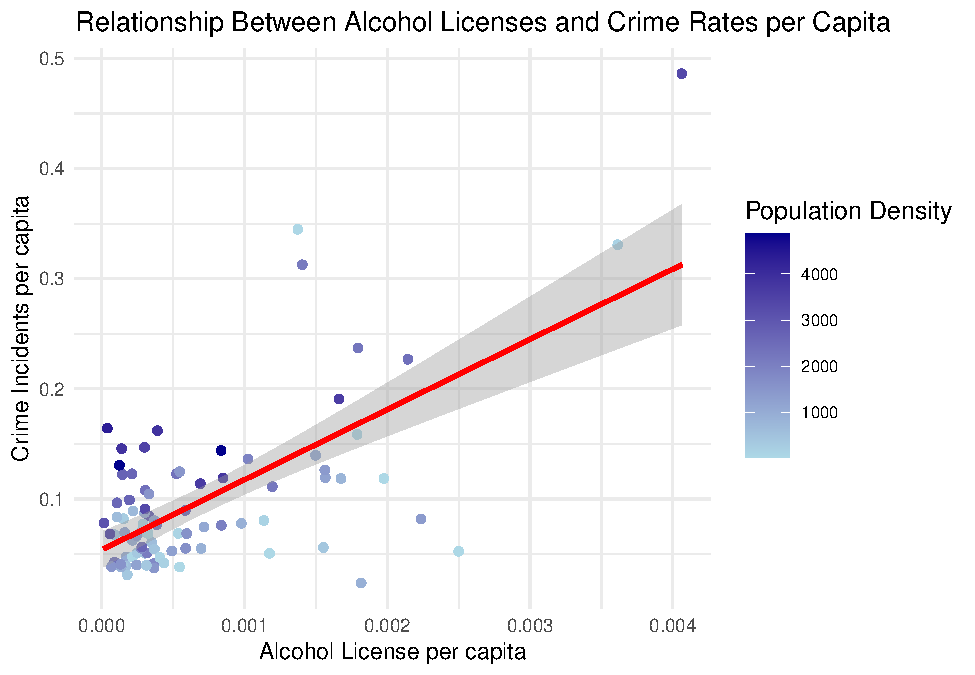
\includegraphics{poli170a_files/figure-latex/unnamed-chunk-4-1.pdf}

\begin{Shaded}
\begin{Highlighting}[]
\FunctionTok{ggsave}\NormalTok{(}\StringTok{"scatterplot\_license\_vs\_crime\_density.png"}\NormalTok{, }\AttributeTok{plot =}\NormalTok{ p, }\AttributeTok{dpi =} \DecValTok{300}\NormalTok{)}
\end{Highlighting}
\end{Shaded}

\begin{verbatim}
## Saving 6.5 x 4.5 in image
## `geom_smooth()` using formula = 'y ~ x'
\end{verbatim}

\end{document}
